\begin{frame}
\frametitle{История развития региона}
\begin{columns}
\column{0.5\textwidth}
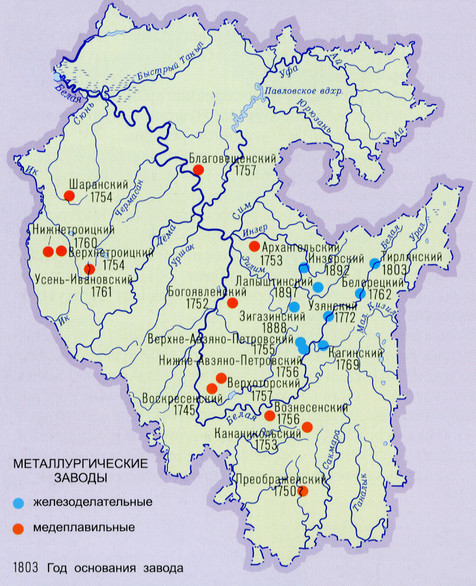
\includegraphics[width=1\linewidth]{pics/sasha/factories_18-19}

\column{0.5\textwidth}
Присоединение территорий республики завершилось к середине XVII века. \\[10pt]

Вторая половина XVII -- массовые восстания. 1773-1775 гг -- Крестьянская война. \\[10pt]

Со второй половины XVIII века начинают сооружаться заводы. \\[10pt]

20 марта 1919 г. -- создана Башкирская Автономная Советская Республика. 
\end{columns}
\end{frame}
%%%%%%%%%%%%%%%%%%%%%%%%%%%%%%%%%%%%%%%%%%%%%%%%%%%%%%%%%%%%%%%%%%%%

%%%%%%%%%%%%%%%%%%%%%%%%%%%%%%%%%%%%%%%%%%%%%%%%%%%%%%%%%%%%%%%%%%%%
\begin{frame}
\frametitle{История развития региона}

В 1920-30-е годы -- рост промышленного производства. 
\begin{center}
\begin{tabular}{|c|c|c|c|c|c|c|c|}
\hline 
Год & 1913 & 1940 & 1950 & 1960 & 1970 & 1980 & 1990 \\ 
\hline 
Темпы роста,\% & 1,0 & 10 & 41 & 186 & 478 & 983 & 1221 \\ 
\hline 
\end{tabular} 
\end{center}

1941 1945 гг. – Великая Отечественная война. Башкортостан стал одним из важнейших регионов перебазирования промышленности страны.

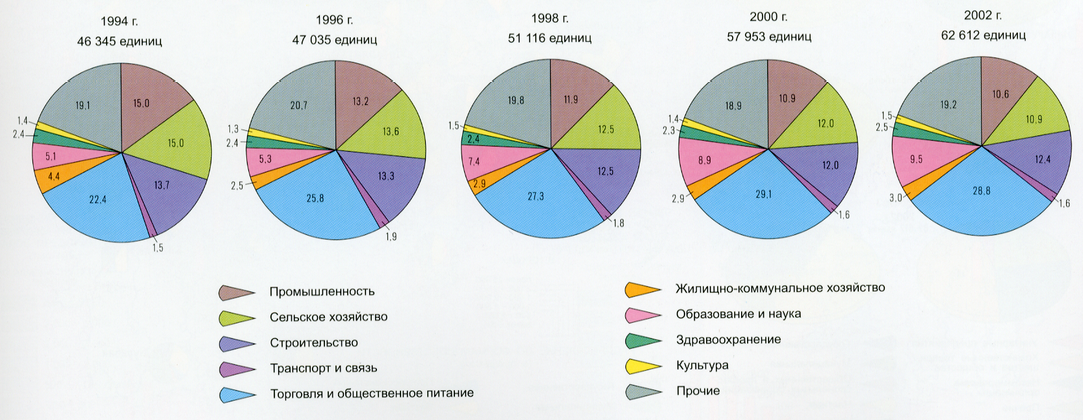
\includegraphics[width=1\linewidth]{pics/sasha/industries}

\end{frame}
%%%%%%%%%%%%%%%%%%%%%%%%%%%%%%%%%%%%%%%%%%%%%%%%%%%%%%%%%%%%%%%%%%%%

%%%%%%%%%%%%%%%%%%%%%%%%%%%%%%%%%%%%%%%%%%%%%%%%%%%%%%%%%%%%%%%%%%%%
\begin{frame}
\frametitle{Отраслевая и территориальная структура экономики}
\begin{columns}
\column{0.5\textwidth}
Центры промышленного производства: 
\begin{itemize}
\item Уфа 
\item Стерлитамак 
\item Салават 
\item Ишимбай 
\item Нефтекамск 
\end{itemize}

\column{0.4\textwidth}
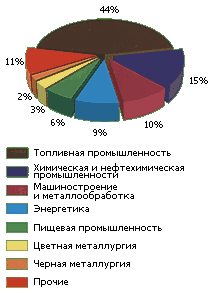
\includegraphics[width=1\linewidth]{pics/sasha/promstruct}
\end{columns}
\end{frame}
%%%%%%%%%%%%%%%%%%%%%%%%%%%%%%%%%%%%%%%%%%%%%%%%%%%%%%%%%%%%%%%%%%%%

%%%%%%%%%%%%%%%%%%%%%%%%%%%%%%%%%%%%%%%%%%%%%%%%%%%%%%%%%%%%%%%%%%%%
\begin{frame}
\frametitle{Отраслевая и территориальная структура экономики}

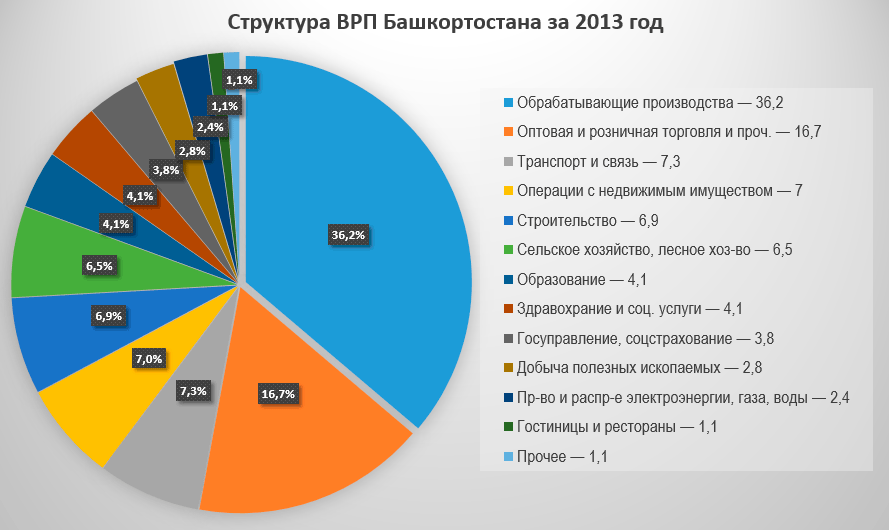
\includegraphics[width=1\linewidth]{pics/sasha/vrp} 

\end{frame}
%%%%%%%%%%%%%%%%%%%%%%%%%%%%%%%%%%%%%%%%%%%%%%%%%%%%%%%%%%%%%%%%%%%%

%%%%%%%%%%%%%%%%%%%%%%%%%%%%%%%%%%%%%%%%%%%%%%%%%%%%%%%%%%%%%%%%%%%%
\begin{frame}
\frametitle{Отраслевая и территориальная структура экономики}

$\blacktriangleright$ Нефтедобыча и нефтехимическая промышленность\\[2pt]

В республике разведано 191 месторождение нефти и газа, из них в разработке находится 161 месторождение. \\[2pt]
Ведущее нефтегазодобывающее предприятие Башкирии — ПАО «Акционерная нефтяная компания „Башнефть“». \\[5pt]

$\blacktriangleright$ Машиностроение и металлообработка
\begin{itemize}
\item производство оборудования для предприятий нефтедобычи, нефте- и газопереработки, химии и нефтехимии: г. Ишимбай, г. Салават
\item вертолестроение: г. Кумертау
\item производство автобусов: г. Нефтекамск 
\item производство троллейбусов: г. Уфа 
\item производство вездеходов: г. Ишимбай
\end{itemize}

\end{frame}
%%%%%%%%%%%%%%%%%%%%%%%%%%%%%%%%%%%%%%%%%%%%%%%%%%%%%%%%%%%%%%%%%%%%

%%%%%%%%%%%%%%%%%%%%%%%%%%%%%%%%%%%%%%%%%%%%%%%%%%%%%%%%%%%%%%%%%%%%
\begin{frame}
\frametitle{Отраслевая и территориальная структура экономики}
\begin{columns}
\column{0.5\textwidth}
$\blacktriangleright$ Пищевая промышленность\\[20pt]
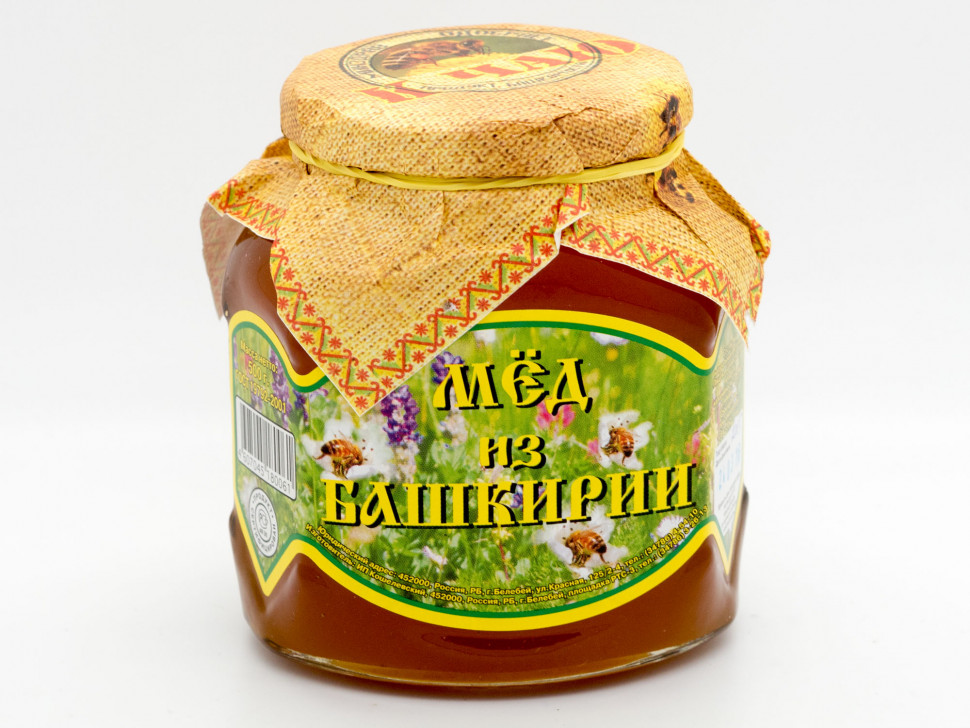
\includegraphics[width=1\linewidth]{pics/sasha/honey}

\column{0.5\textwidth}
$\blacktriangleright$ Энергетика\\[2pt]
\begin{itemize}
\item ТЭК: 50\% общерегионального объёма отгруженной продукции, 70\% полученной прибыли, 40\% поступлений в бюджет республики, более 30\% инвестиций в основной капитал и 80\% валютных поступлений
\item 31 электростанция
\item 3 солнечные электростанции
\end{itemize}
\end{columns}
\end{frame}
%%%%%%%%%%%%%%%%%%%%%%%%%%%%%%%%%%%%%%%%%%%%%%%%%%%%%%%%%%%%%%%%%%%%

%%%%%%%%%%%%%%%%%%%%%%%%%%%%%%%%%%%%%%%%%%%%%%%%%%%%%%%%%%%%%%%%%%%%
\begin{frame}
\frametitle{Отраслевая и территориальная структура экономики}

$\blacktriangleright$ Сельское хозяйство
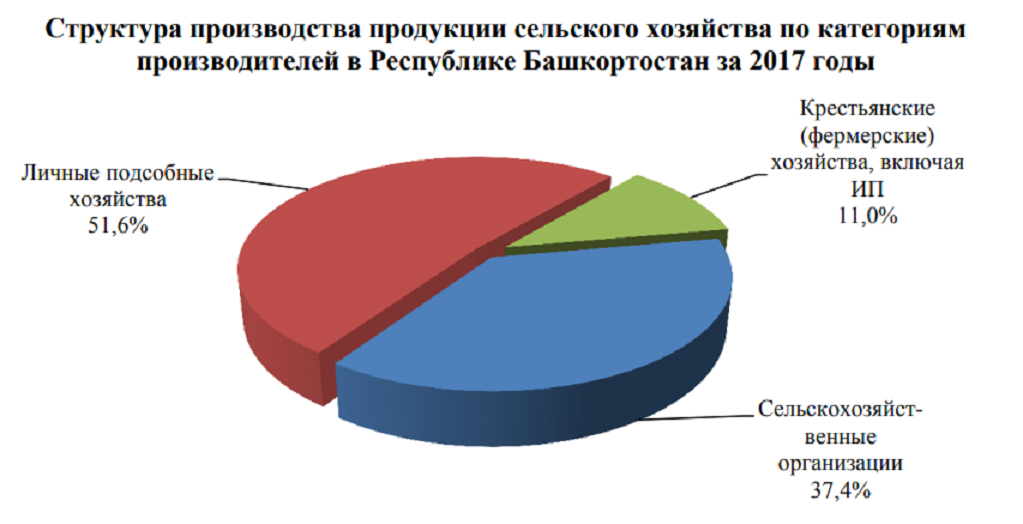
\includegraphics[width=1\linewidth]{pics/sasha/agriculture_struct}

\end{frame}
%%%%%%%%%%%%%%%%%%%%%%%%%%%%%%%%%%%%%%%%%%%%%%%%%%%%%%%%%%%%%%%%%%%%

%%%%%%%%%%%%%%%%%%%%%%%%%%%%%%%%%%%%%%%%%%%%%%%%%%%%%%%%%%%%%%%%%%%%
\begin{frame}
\frametitle{Отраслевая и территориальная структура экономики}

$\blacktriangleright$ Торговля\\[20pt]
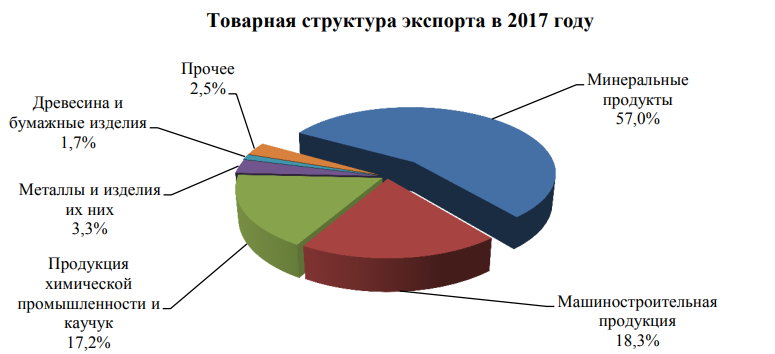
\includegraphics[width=1\linewidth]{pics/sasha/export}

\end{frame}
%%%%%%%%%%%%%%%%%%%%%%%%%%%%%%%%%%%%%%%%%%%%%%%%%%%%%%%%%%%%%%%%%%%%

%%%%%%%%%%%%%%%%%%%%%%%%%%%%%%%%%%%%%%%%%%%%%%%%%%%%%%%%%%%%%%%%%%%%
\begin{frame}
\frametitle{Отраслевая и территориальная структура экономики}

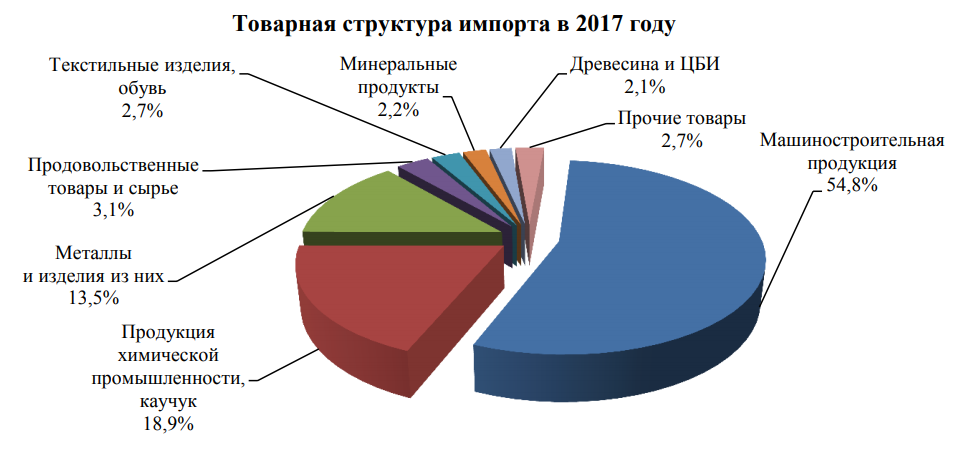
\includegraphics[width=1\linewidth]{pics/sasha/import}

\end{frame}
%%%%%%%%%%%%%%%%%%%%%%%%%%%%%%%%%%%%%%%%%%%%%%%%%%%%%%%%%%%%%%%%%%%%
